%**************************************************************************
%*
%*  Paper: ``INSTRUCTIONS FOR AUTHORS OF LATEX DOCUMENTS''
%*
%*  Publication: 2026 Winter Simulation Conference Author Kit
%*
%*  Filename: wsc26paper.tex
%*
%*  Date: January 14, 2026
%*
%*  Word Processing System: TeXstudio
%*
%**************************************************************************


\documentclass{wscpaperproc}
\usepackage{latexsym}
%\usepackage{caption}
\usepackage{graphicx}
\usepackage{mathptmx}
\usepackage[T1]{fontenc}


%
%****************************************************************************
% AUTHOR: You may want to use some of these packages. (Optional)
\usepackage{amsmath}
\usepackage{amsfonts}
\usepackage{amssymb}
\usepackage{amsbsy}
\usepackage{amsthm}
%****************************************************************************


%
%****************************************************************************
% AUTHOR: If you do not wish to use hyperlinks, then just comment
% out the hyperref usepackage commands below.

%% This version of the command is used if you use pdflatex. In this case you
%% cannot use ps or eps files for graphics, but pdf, jpeg, png etc are fine.

\usepackage[pdftex,colorlinks=true,urlcolor=blue,citecolor=black,anchorcolor=black,linkcolor=black]{hyperref}

%% The next versions of the hyperref command are used if you adopt the
%% outdated latex-dvips-ps2pdf route in generating your pdf file. In
%% this case you can use ps or eps files for graphics, but not pdf, jpeg, png etc.
%% However, the final pdf file should embed all fonts required which means that you have to use file
%% formats which can embed fonts. Please note that the final PDF file will not be generated on your computer!
%% If you are using WinEdt or PCTeX, then use the following. If you are using
%% Y&Y TeX then replace "dvips" with "dvipsone"

%%\usepackage[dvips,colorlinks=true,urlcolor=blue,citecolor=black,%
%% anchorcolor=black,linkcolor=black]{hyperref}
%****************************************************************************


%
%****************************************************************************
%*
%* AUTHOR: YOUR CALL!  Document-specific macros can come here.
%*
%****************************************************************************

% If you use theoremes
\newtheoremstyle{wsc}% hnamei
{3pt}% hSpace abovei
{3pt}% hSpace belowi
{}% hBody fonti
{}% hIndent amounti1
{\bf}% hTheorem head fontbf
{}% hPunctuation after theorem headi
{.5em}% hSpace after theorem headi2
{}% hTheorem head spec (can be left empty, meaning `normal')i

\theoremstyle{wsc}
\newtheorem{theorem}{Theorem}
\renewcommand{\thetheorem}{\arabic{theorem}}
\newtheorem{corollary}[theorem]{Corollary}
\renewcommand{\thecorollary}{\arabic{corollary}}
\newtheorem{definition}{Definition}
\renewcommand{\thedefinition}{\arabic{definition}}

%%% TREATMENT OF FIGURES -----------------------------------------------------------------------------
    % Alter some LaTeX defaults for better treatment of figures:
    % See p.105 of "TeX Unbound" for suggested values.
    % See pp. 199-200 of Lamport's "LaTeX" book for details.
    %   General parameters, for ALL pages:
    \renewcommand{\topfraction}{0.9}     % max fraction of floats at top
    \renewcommand{\bottomfraction}{0.8}             % max fraction of floats at bottom
    %   Parameters for TEXT pages (not float pages):
    \setcounter{topnumber}{2}
    \setcounter{bottomnumber}{2}
    \setcounter{totalnumber}{4}     % 2 may work better
    \renewcommand{\textfraction}{0.05}  % allow minimal text w. figs
    %   Parameters for FLOAT pages (not text pages):
    \renewcommand{\floatpagefraction}{0.85}      % require fuller float pages
                % N.B.: floatpagefraction MUST be less than topfraction !!
    \renewcommand{\dblfloatpagefraction}{0.85} % require fuller float pages

%#########################################################
%*
%*  The Document.
%*
\begin{document}

%***************************************************************************
% AUTHOR: AUTHOR NAMES GO HERE
% FORMAT AUTHORS NAMES Like: Author1, Author2 and Author3 (last names)
%
%		You need to change the author listing below!
%               Please list ALL authors using last name only, separate by a comma except
%               for the last author, separate with "and"
%
\WSCpagesetup{LastName1, LastName2, LastName3, LastName4, and LastName (LastAuthor)}

% AUTHOR: Enter the title, all letters in upper case
\title{INSTRUCTIONS FOR AUTHORS OF PAPERS USING \LaTeX}

% AUTHOR: Enter the authors of the article, see end of the example document for further examples
\author{\begin{center}Varun Ramamohan\textsuperscript{1}, Anatoli Djanatliev\textsuperscript{2}, Masoud Fakhimi\textsuperscript{3}, Caroline Krejci\textsuperscript{4}, and Cristina Ruiz Martin\textsuperscript{5}\\
[11pt]
\textsuperscript{1}Dept.~of Mechanical Eng., Indian Institute of Technology Delhi, New Delhi, INDIA\\
\textsuperscript{2}Dept.~of Computer Science, University of Applied Sciences Ingolstadt, Ingolstadt, GERMANY\\
\textsuperscript{3}University of Surrey, Surrey Business School, Guildford, Surrey, UK\\
\textsuperscript{4}Industrial, Manufacturing and Systems Eng., University of Texas at Arlington, Arlington, TX, USA\\
\textsuperscript{5}Systems and Computer Eng., Carleton University, Ottawa, ON, CANADA\end{center}
}

\maketitle

\vspace{-12pt}

\section*{ABSTRACT}
This document provides instructions for producing a proceedings paper for the 2026 Winter Simulation Conference (WSC) with \LaTeX. It also serves as a sample file that you can edit to prepare your submission, and a checklist to ensure that your submission meets the WSC 2026 requirements. Please follow the guidelines provided in this document when preparing your paper. Failure to do so may lead to your paper being rejected, returned for appropriate revision, or edited without your prior knowledge.


\section{INTRODUCTION}
\label{sec:intro}

This paper provides instructions for the preparation of papers for the 2026
Winter Simulation Conference (WSC) using \LaTeX. There is a companion paper that
provides instructions for the preparation of papers using Microsoft Word. \textbf{The easiest way to write a paper using \LaTeX\ that complies with the
requirements is to edit the source file, {\tt wsc26paper.tex}, for this document.}
Do not use an older version, as \textit{some specifications have changed}.
The style of this document is based on the special paper class file {\tt wscpaperproc} which is selected by using {\tt $\backslash$documentclass\{wscpaperproc\}}.

An author kit is available online via the \href{http://www.wintersim.org}%
{conference website}.
The author kit includes this \LaTeX\ document and its Microsoft Word companion.
It also includes guidelines that you may find helpful for writing a conference paper and for giving a presentation.

This document was typeset using {\tt pdflatex}, which allows you to use certain
graphics file types that are not allowed using the outdated {\tt latex-dvips-ps2pdf} route.
For more on this issue, see Section~\ref{sec:graphics} below.

\section{GENERAL GUIDELINES}

\subsection{Language}
The paper should be prepared using U.S. English in the interest of consistency across the proceedings. Please carefully check the spelling of words before you submit your paper. There are spell checkers for \LaTeX\ as well.
Some examples of software which supports spell checking are TexnicCenter, TexMaker, and TexClipse.

\subsection{Paper Submission}
You will submit the Portable Document Format ({\tt .pdf}) of your paper electronically at the \href{http://www.wintersim.org}{conference website}. Source files (text, graphics, bib) are not needed. If the paper is accepted, you will electronically submit the \LaTeX source file ({\tt .tex}) for the final version of your paper in a ZIP format that includes all figures and auxiliary files.
The editors may send the file back to you with the request to make changes to conform to conference guidelines. For minor changes, the editors may make the changes themselves. Final {\tt .pdf} files are generated by the conference proceedings editors.

You will also need to transfer the copyright of your article to the WSC using the copyright transfer form that will be available via the conference web site at the appropriate time. {\em For your paper to be published by the WSC, you must complete the transfer of copyright.}
When you have successfully transferred the copyright, you will receive a {\tt .pdf} receipt.

If you are unable to satisfy these requirements, you should contact the proceedings editors.

\subsection{Objectivity}
The content of the paper should be objective and without any appearance of commercialism. In general, comparisons of commercial software should be avoided unless they are central to the topic. If a comparison of commercial software is included, it should be based on objective analysis that includes criteria, description of ranking methodology on each criterion, and the rankings themselves to arrive at a conclusion. If an approach other than a detailed objective analysis is used to select the simulation software used for the study being reported, such as, availability of the software, or the familiarity of the analyst with the software, it should be clearly identified.

\subsection{Length Constraints}

\subsubsection{Length of the Abstract}
The abstract should be at most 150 words. Since abstracts of all papers accepted for publication in the proceedings will also appear in the final program, the length limit of 150 words will be strictly enforced for each abstract. The abstract should consist of a single paragraph, and it should not contain references or mathematical symbols. Do not include a list of keywords. Keywords are not used in WSC proceedings.

\subsubsection{Length of the Paper}
The page size in the proceedings must be 8.5 inches by 11 inches (21.6 cm by 27.9 cm). The overall length of the paper should be at least 5 proceedings pages. \textbf{Papers should be at most twelve (12) pages,} except for introductory tutorials, advanced tutorials, and panel sessions, for which the limit is 15 pages. Exceeding the page limit will result in rejection for the proceedings.

\subsection{Font Specification and Spacing}
The paper should be set in the Times New Roman font using a 11-point font size. The paper should be single spaced. Do not use other fonts; use of other fonts means the proceedings editors will need to send the paper back to you to change the font.

\subsection{Margins}
\label{sec:margins}
The width of the text area is 6.5 inches (16.5 cm). The left and right margins should be 1 inch (2.54 cm) on each page. Except for the first page, the top and bottom margins should be 1 inch (2.54 cm). First page has 1.5 inch (3.81 cm) margin from the title to the top of the page, and 1 inch bottom margin. Authors should neither change the header and footer settings nor the corresponding \LaTeX\ style when preparing a manuscript.

\subsection{Justification}
Headings of sections, subsections, and subsubsections should be left-justified. One-line captions for figures or tables should be centered. A multiline caption for a figure or table should be fully justified. All other text should be fully justified across the page (that is, the text should line up on the right-hand and left-hand sides of the page).

\subsection{Headings of Sections, Subsections, and Subsubsections}
Section, subsection, and subsubsection headings should appear flush left, set in the bold font style, and numbered as shown in this document. The headings for the Abstract, Acknowledgments, References and Author Biographies sections are not numbered. Section headings should be set in \textbf{FULL CAPITALS LIKE THIS PHRASE}, while subsection and subsubsection headings should be \textbf{Capitalized in Headline Style like This Phrase}. Lengthy headings should be broken across two or more lines. \textbf{Again, these formats should be accomplished using section, subsection, subsubsection, etc.}

\subsubsection{Paragraphs}
The first paragraph after a heading should not be indented; all other paragraphs should be indented by 0.25 inches (0.63 cm). Do not insert additional space between paragraphs.

Programming code should use ``Program Start'', ``Program'', and ``Program End'' Styles with the following guidelines.

\begin{verbatim}
class Exponential{
...// Properties of the Exponential
};
\end{verbatim}

One-line programs should use the ``Program Both'' style.

\begin{verbatim}
Exponential interArrival;
\end{verbatim}

\subsubsection{Footnotes}
\textbf{Do not use footnotes}; instead incorporate such material into the text directly or parenthetically.

\subsubsection{Page Numbers}
Do not include page numbers. Page numbers are generated by the proceedings editors once all accepted papers are ordered for the final proceedings.

\section{FORMATTING THE FIRST PAGE}

\subsection{Running Heads}
The running head (provided in the template) in the upper left-hand corner of the first page (which should read {\em \currentCaption}\dots) is left-justified and set in the 11-point italic font style. You do not have to change the content of the first-page header; the first-page header was set by the proceedings editors in the preparation of this document.

Running heads on the second and subsequent pages should contain the last names of the authors, centered and set in the 11-point italic font style. For example, running heads for papers would appear like \textit{Justme} for papers with one author, or \textit{Justme and Him} for papers with two authors, or \textit{Justme, Him, and Youtoo} for papers with three authors, etc. These are created by using the macro\newline

\begin{verbatim}
\WSCpagesetup{LastName1, LastName2, and LastNameLastAuthor}

\end{verbatim}
defined in the class file.
Please use this macro to set up the running heads, as it sets further parameters important for the correct layout of the document.

The author names are listed in the same order as they appear on the title page, which is the same order the author biographies are provided.
These entries {\bf do} need to be changed by the authors in the {\tt $\backslash$WSCpagesetup} command in the source for this file.
Please give all author names and do not use \textit{et al.}, except in the rare situation where they don't fit on one line. In the latter case, only the first author is given followed by ``et al.''.


\subsection{Title and Authors}
Center the title of the paper across the page and set it in bold {\bf FULL CAPITALS} so that the top edge of the title begins 1.5 inches from the top of the page.
The correct placement is automatically done by the class file as well.
Just use the {\tt $\backslash$title} and {\tt $\backslash$maketitle} commands as it is done in the source of this document.
Multiline titles should have about the same amount of text on each line.

There should be 2 blank lines between the title and the authors' names (will be inserted by the class file if the {\tt $\backslash$author}, {\tt $\backslash$title}, and {\tt $\backslash$maketitle} commands are used).

All authors' names should have initial letters capitalized, and be listed on a line in a centered fashion, with the author's first name first and no job title or honorific. In the case of many authors, multiple centered lines might be used to list all authors. Behind each author's name is superscript \textsuperscript{1}, \textsuperscript{2}, \textsuperscript{3}, etc. denoting the author's affiliation. If an author has multiple affiliations, then only the main affiliation should be listed unless it is strictly necessary to use multiple affiliations, in which case the superscript could consist of multiple indices, e.g., \textsuperscript{1,2}. On the other hand, each affiliation could apply to multiple co-authors.
These affiliations are detailed under the authors' names, with one blank line between authors' names and the affiliation details. Each affiliation starts with the superscript index, then the department, institution, city, standard two-letter state or province abbreviation, and country. The state abbreviation and country name should be in FULL CAPITALS.
Each affiliation should be detailed in a single centered line to the extent possible, by using common abbreviations, e.g., ``Dept.'' for ``Department'', ``Eng.'' for ``Engineering'' and other common-sense abbreviations if needed. However, using multiple lines is acceptable if a single line is not sufficient to detail the affiliation even after a reasonable effort to abbreviate.
For papers with multiple authors, the authors should be listed in order of decreasing contribution. Some examples of title page heading and common-sense abbreviations are shown in Figures~\ref{fig:different}--\ref{fig:two lines} and Table~\ref{table:abbreviation} respectively at the end of this document. There should be two blank lines between the author fields and the text of the paper. Do not include email addresses on the first page; emails for authors are provided in the author biographies.


You should use the {\tt $\backslash$author} command to enter author names -- see the source for this document.

\section{FORMATTING SUBSEQUENT PAGES}
Please refer to Section~\ref{sec:margins} for the correct margins.

\subsection{Mathematical Expressions in Text and in Displays}
Display only the most important equations, and number only the displayed equations that are explicitly referenced in the text.
To conserve space, simple mathematical expressions such as $\bar Y = n^{-1} \sum_{i=1}^n Y_i$ may be incorporated into the text.
Mathematical expressions that are more complicated or that must be referenced later should be displayed, as in
$$s^2 = \frac 1 {n-1} \sum_{i=1}^n (Y_i - \bar Y)^2.$$

If a display is referenced in the text, then enclose the equation number in parentheses and place it flush with the right-hand margin of the
column. For example, the quadratic equation has the general form

\begin{equation} \label{eq:quadratic}
ax^2 + bx + c = 0, \mbox{ where } a \ne 0.
\end{equation}

In the text, each reference to an equation number should also be enclosed in parentheses. For example, the solution to (\ref{eq:quadratic}) is given in (\ref{eq: quadratic sol}) in Appendix \ref{app:quadratic}.

If the equation is at the end of a sentence, then you should end the equation with a period. If the sentence in question continues beyond the equation, then you should end the equation with the appropriate punctuation -- that is, a comma, semicolon, or no punctuation mark. If the equation is not included within any sentence, but just given between two paragraphs, no punctuation is used as in equation (\ref{eq:quadratic_second}).

\begin{equation} \label{eq:quadratic_second}
ax^2 + bx + c = 0
\end{equation}

\subsection{Displayed Lists}
A displayed list is a list that is set off from the text, as opposed to a run-in list that is incorporated into the text. The bulleted list given below provides more information about the format of a displayed list.

\begin{itemize}
	\item Use standard bullets instead of checks, arrows, etc.\ for bulleted lists.
\end{itemize}
\begin{enumerate}
	\item For numbered lists, the labels should not be arabic numerals enclosed in parentheses because such labels cannot be distinguished from equation numbers.
\end{enumerate}

Indent the paragraph after the list.

\subsection{Figures and Tables}
\label{sec:graphics}
Figures and tables should be centered within the text and should not extend beyond the right and left margins of the paper.
Figures and tables can make use of color since the WSC produces electronic proceedings.
However, try to select colors that can be differentiated when printing in black and white in consideration of people using such printers. Figures and tables are numbered sequentially, but separately, using arabic numerals.
All tables and figures should be explicitly referenced in the text and they should not be placed before they are referenced.
The reference is always written in full (Figure 1), and never abbreviated as in ``(Fig. 1)''.
For figures which can fit next to each other, the author can choose to align them next to each other with the figure text centered below each figure and on the same line for both figures. For tables which can fit next to each other, the author can also choose to align them next to each other with the table text centered above each table and on the same line for both tables.

The table's one-line captions are centered, while multi-line captions are fully justified.
The captions appear {\em above} the table.
Captions can be written using normal sentences with full punctuation. All captions should end with a period. It is fine to have multiple-sentence captions that help to explain the table.
See Tables \ref{tab: first} and \ref{tab: second} for examples.

\begin{table}[htb]
\centering
\caption{Table captions appear above the table, and if they are longer than one line they are fully justified. Captions are written using normal sentences with full punctuation. It is fine to have multiple-sentence captions that help to explain the table.\label{tab: first}}
\begin{tabular}{rll}
\hline
Creature & IQ & Diet\\ \hline
dog & 70 & anything\\
human & 60 & ice cream \\
dolphin & 120 & fish fillet\\
\hline
\end{tabular}
\end{table}

\begin{table}[htb]
\centering
\caption{Comparison between samples.\label{tab: second}}
\begin{tabular}{|r|l|}
\hline
Sample & Height (cm) \\ \hline
Plant one & 50 \\ \hline
Plant two & 58 \\
\hline
\end{tabular}
\end{table}

Captions end with a period. One-line captions are centered, while multiline captions are fully justified. Figure captions appear below the figure. See Figures \ref{fig: tahi} and \ref{fig: rua} for examples.

\begin{figure}[htb]
{
\centering
%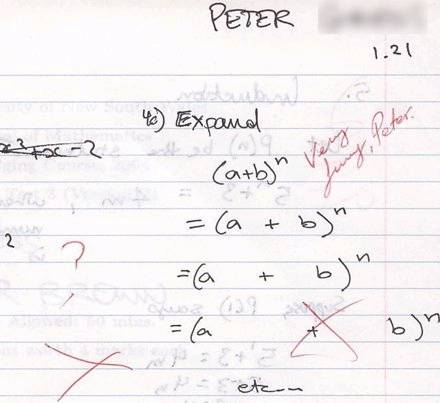
\includegraphics[width=0.9\columnwidth]{MathExpandExpression.jpg}
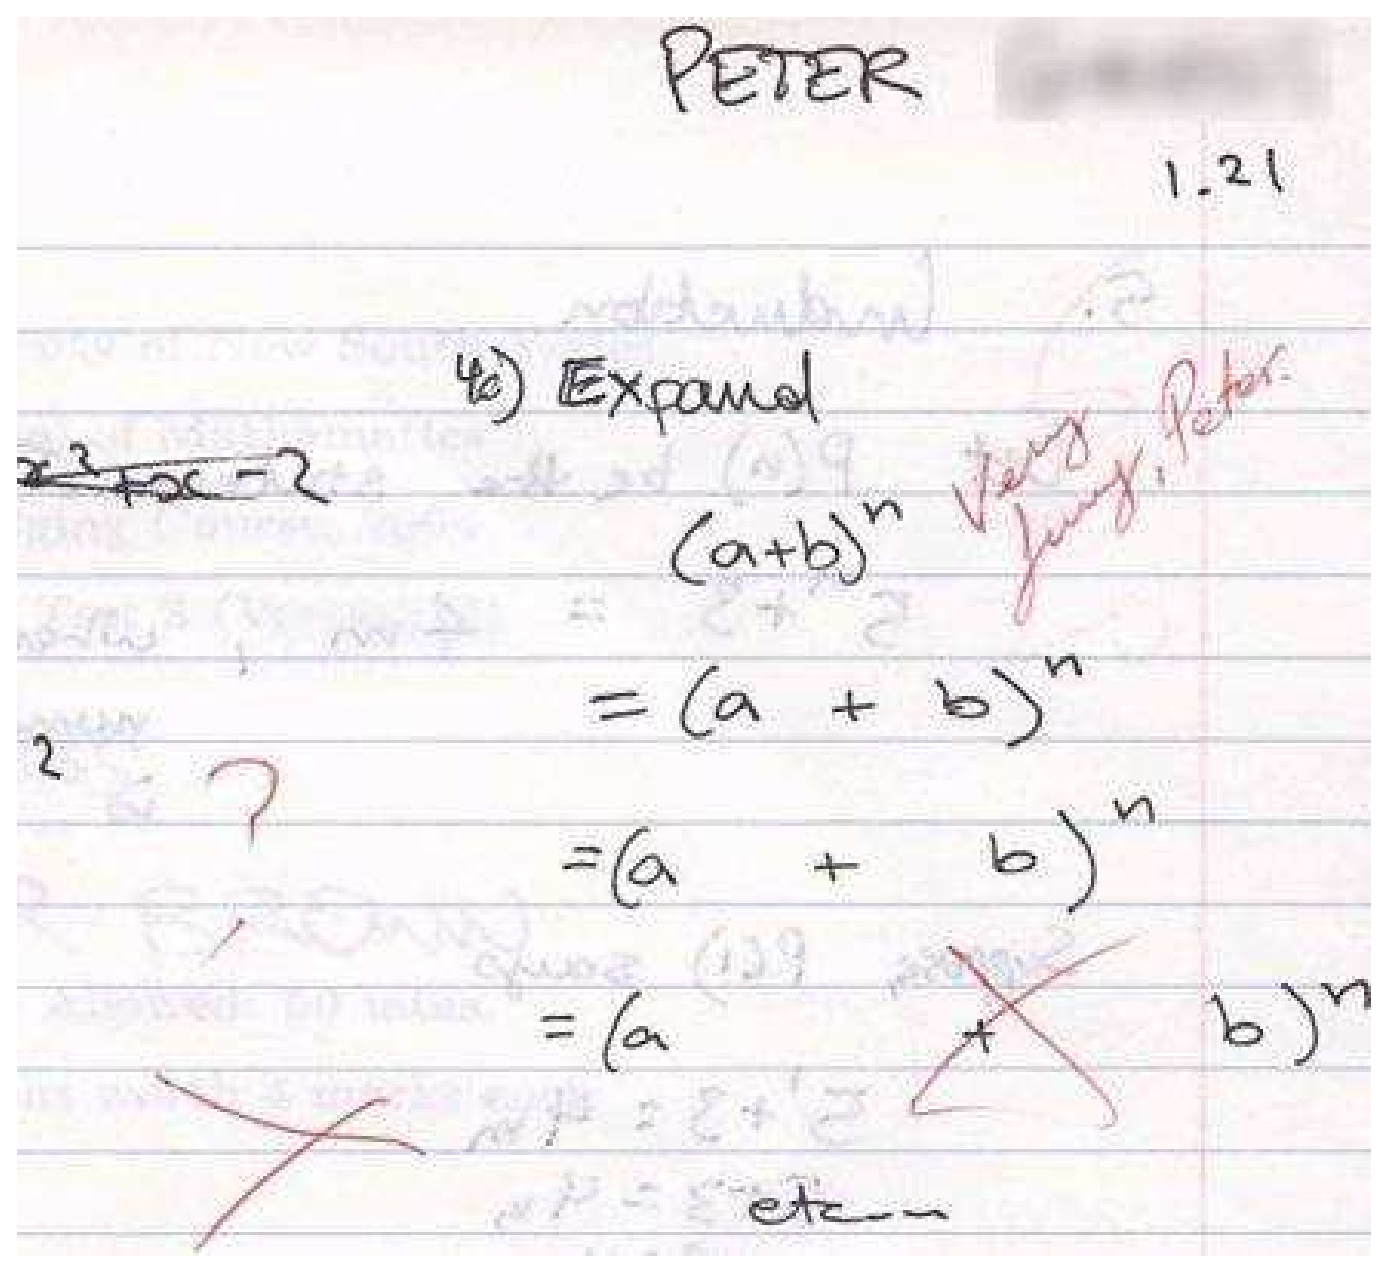
\includegraphics[width=0.50\textwidth]{MathExpandExpression}
\caption{An unusual answer to a question.\label{fig: tahi}}
}
\end{figure}

\begin{figure}[htb]
{
\centering
%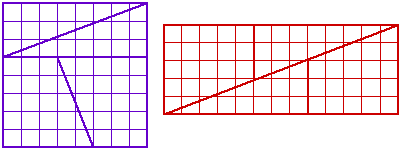
\includegraphics[width=0.9\columnwidth]{puzzle.png}
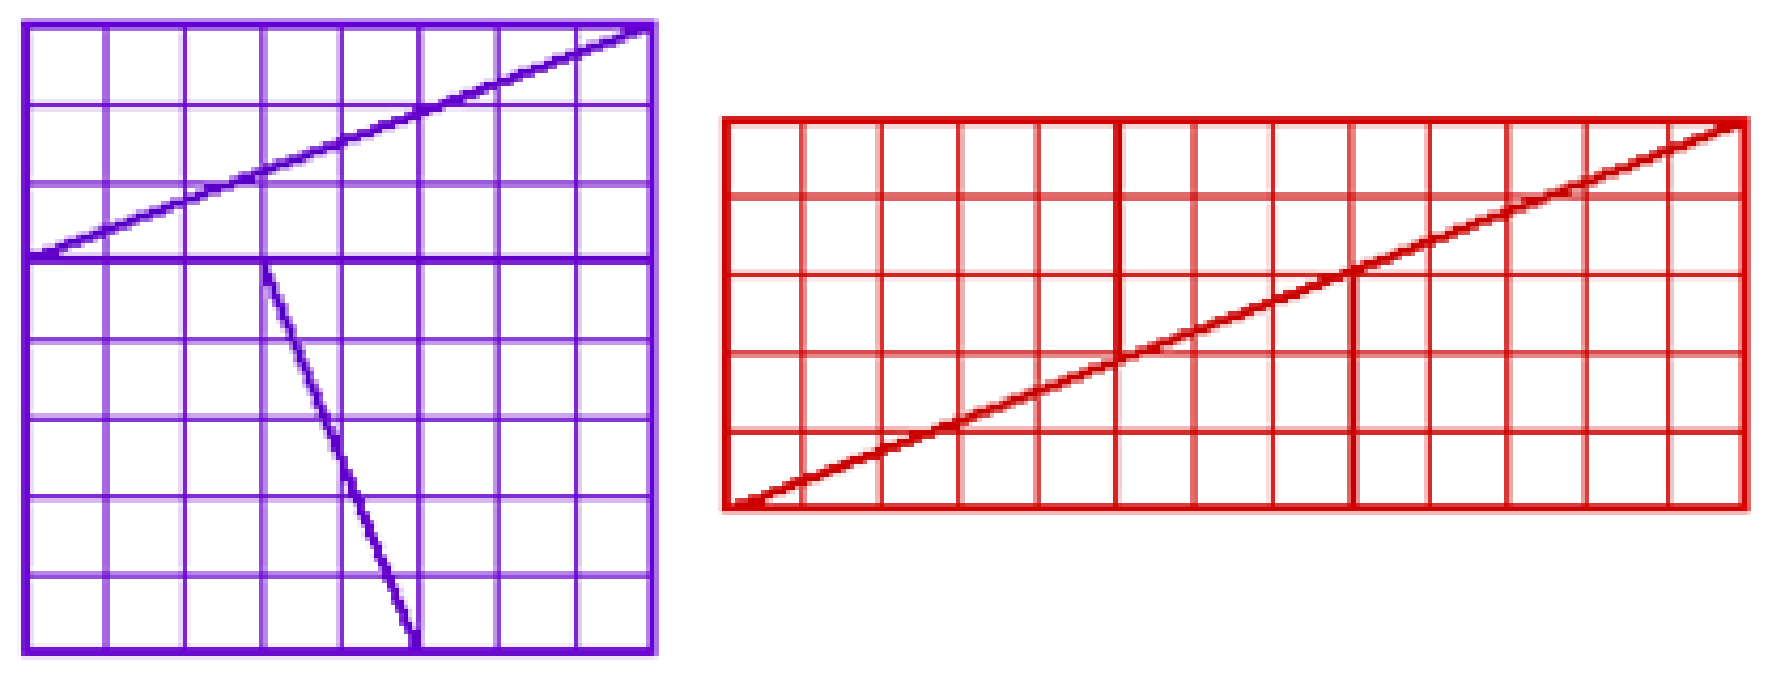
\includegraphics[width=0.50\textwidth]{puzzle}
\caption{The area of the square is 64 squares, while that of the rectangle is 65 squares, yet they are made of the same pieces! How
is this possible? \label{fig: rua}}
}
\end{figure}

References to tables and figures identified by number are capitalized. Avoid using ``in the previous table'' or ``in the figure below'', as positions might change in the final formatting. Be sure to use the {\tt $\backslash$label} command within the figure or table environment and refer to the associated figure or table using {\tt Table$\sim \backslash$ref\{labelgiven\}}.
Please do not use hard coded figure/table numbers. This is error prone, and the references will not be hyperlinks.

Please ensure that the text within figures uses standard fonts and is readable: Arial (recommended), Symbol, etc. The minimum font size should be around 9pt (Arial). Remember that you might need larger fonts in your original figure if you reduce the size of the figure in your WSC paper to less that 100\% (e.g., when you insert your figure with a 50\% of its original size, your original fonts have to be $>=$18pt). This applies to all text elements in the figure, including captions of axes, etc.

Including graphics files in your document can be complicated.
Use {\tt .jpg}, {\tt .png} or {\tt .pdf} files.
The main difference between the formats is how they store the images and how well suited they are for specific graphics. You can choose between bitmap and vector graphics.
Bitmap graphics are well suited for photographs (jpg is very common here) or for screenshots (PNG is a lossless encoding in contrast to jpg, and is thus better suited for all those cases where you have sharp edges in your graphics).
Vector graphics are the encoding to be chosen for all kinds of drawings (diagrams, charts, ...). In contrast to bitmap formats, they can be scaled to any size without any loss of sharpness. This makes it possible to read such graphics even if two pages are printed on one sheet of paper, or if the documents are read electronically.
So what to choose for your \LaTeX\ document? As a rule of thumb you should always prefer PDF or PS and EPS.
In general these three encodings can contain both, bitmap and vector graphics. But there is no need (and no use) to convert your bitmaps to any of these.

Use the {\tt PDFLaTeX} command to generate your pdf file, as was done with this file.
The final file format is PDF.
If you include figures via {\tt includegraphics}, then please do so without the file ending (e.g., skip .pdf, .ps, ...).

\subsection{Definitions and Theorems}
Definitions, theorems, propositions, etc. should be formatted like a normal paragraph with boldface heading as shown in the examples below. Number
these items separately and sequentially. You may choose not to separately number theorems, propositions, corollaries, etc., as opposed to the example below where corollaries and theorems are numbered together. Search the source of this document to see how these environments were defined. The key
command is {\tt $\backslash$newtheorem}. Do not use a period after the definition, theorem, corollary or proposition \textit{number}, but do end the sentence with a period.

\begin{definition}
In colloquial New Zealand English, the term {\em dopey mongrel} is used to refer to someone who has exhibited less than stellar intelligence.
\end{definition}

\begin{theorem}
If a proceedings editor from New Zealand accidentally deletes his draft of the author kit shortly after completing it, he would be considered to be a dopey mongrel.
\end{theorem}

\begin{corollary}
One of the proceedings editors is a dopey mongrel.
\end{corollary}

Indent the paragraph after the definition or theorem.

\subsection{Hyperlinks}
\label{sec: hyper}
A {\em hyperlink} specifies a web address (URL) or an email address.
The use of hyperlinks allows authors for providing readers access to external electronic information, such as a dynamic simulation or animation.
The use of hyperlinks is at the discretion of the author(s).
{\bf While the use of hyperlinked text is encouraged in the main body of the paper, it is recommended that corresponding web addresses and other identifying information should be provided in the list of references.}
For example, instead of spelling out the web address of the conference website, one would refer to the \href{http://www.wintersim.org}{conference website}~\cite{WSC}, and the corresponding entry in the reference section will spell out the associated web address and other relevant information such as author(s) and/or the organization that published the content.
This would allow readers for searching for the content using the author(s), organization, etc. if the actual web address is changed. This also allows for a cleaner appearance of the main body of the paper.

If the author(s) feel that sufficient information is provided in the main body of the paper to locate the content even if the web address is changed, the address can be included in the main body of the paper itself.

Each hyperlink should be set in the same font as the text.
Hyperlinks are {\em not} underlined.
A live hyperlink (or hot link) -- that is, a hyperlink that will activate your web browser and take it to an external web site or that will activate your email software for sending a message to a specific email address -- should be colored blue. You have already seen examples of such hyperlinks in this paper.
To use live hyperlinks in a proceedings paper, use the {\tt hyperref} package. If you are using {\tt PDFLaTeX} to generate your pdf file then, as
was done for this file, you should add the following as the last {\tt $\backslash$usepackage} command in the preamble.\newline


\begin{verbatim}
\usepackage[pdftex,colorlinks=true,urlcolor=blue,citecolor=black,
anchorcolor=black,linkcolor=black]{hyperref}
\end{verbatim}\vspace{5 mm}

\noindent On the other hand, if you are using the traditional {\tt latex - dvips - ps2pdf} route, then users of MiKTeX or PCTeX for Windows should add the command\newline


\begin{verbatim}
\usepackage[dvips,colorlinks=true,urlcolor=blue,citecolor=black,
anchorcolor=black,linkcolor=black]{hyperref}
\end{verbatim}\vspace{5 mm}


\noindent as the last {\tt $\backslash$usepackage} command in the preamble, while users of Y\&Y TeX should add the command\newline


\begin{verbatim}
\usepackage[dvipsone,colorlinks=true,urlcolor=blue,citecolor=black,
anchorcolor=black,linkcolor=black]{hyperref}
\end{verbatim}\vspace{5 mm}


\noindent as the last {\tt $\backslash$usepackage} command in the preamble.
(In general the {\tt $\backslash$usepackage} command above that works for MiKTeX running on a Windows system should also work for most implementations of \LaTeX\ running on a Unix or Apple system.)
Thus the hypertext link \href{http://www.wintersim.org}{conference website}~\cite{WSC} to the WSC website can be established by the command\newline

\begin{verbatim}
\href{http://www.wintersim.org}{conference website}
\end{verbatim}\vspace{5 mm}


\noindent This is especially important since WSC papers are filed in the IEEE Xplore digital library, which does not allow hyperlinks, so for that purpose the hyperlinks are removed.
Therefore it is recommended to add all hypertext references to the {\tt .bib} file and to refer to them from the text as it is done in the example above.
All live hyperlinks still appear in the CD of the proceedings and in other repositories.

If you use the package {\tt hyperref} as suggested here, and if you use citation commands to handle references, then your citations will
become hyperlinks (as in this document).

Non-live hyperlinks -- that is, the hyperlinks that are included for the reader's information but do not actually invoke the reader's web browser or email software should be colored black.

\subsection{Citing a Reference}
To cite a reference in the text, use the author-date method. Thus, \citeN{chi89} could also be cited parenthetically \cite{chi89}.
Do not use a comma within this parenthesis.
For a work by three or more authors, use an abbreviated form. For example, a work by Banks, Carson, and Nelson would be cited in one of the following ways: \shortciteN{bcnn:simulation} or \shortcite{bcnn:simulation}.

Parenthetical citations are enclosed in parentheses $(~)$, not square brackets $[~]$.
Semicolons separate the items in a series of such citations.

The following is a list of correct forms of citations:
\begin{itemize}
\item Brown and Edwards (1993)
\item (Brown and Edwards 1993)
\item (Smith 1987; Brown and Edwards 1992; Brown et al. 1995)
\end{itemize}

The following is a list of \textbf{incorrect} forms of citations:
\begin{itemize}
\item Brown and Edwards [1993]
\item (Brown and Edwards, 1993)
\item (Smith, 1987; Brown and Edwards, 1993)
\item (Smith 1987, Arnold, Brown and Edwards 1992, Brown et al. 1995)
\end{itemize}

\subsection{General Style and Sequence of References}
Place the list of references after the appendices. The section heading is {\bf REFERENCES}, and it is not numbered. List only references that are cited in the text. Do not number the references. The only exception are papers in the ``tutorial'' tracks: Here it is permitted to have an additional section heading {\bf ADDITIONAL READING} after references, followed by further literature that is recommended for continued studies but not directly used within the text of the paper

Do not number the references and arrange them in the following order:
\begin{itemize}
	\item By the last name of the first author.
	\item For papers with the same first author, arrange first all papers by this author only, then all papers by this author and one co-author, and finally all papers with this author and two or more co-authors.
\item Within this sorting sequence, arrange papers by year.
\end{itemize}

To identify multiple references by the same authors and year, append a lower case letter to the year of publication; for example, 1984a and 1984b. The same applies to references that have more than two authors and the same first author and year.

Give complete references without abbreviations. List \underline{all} authors except when there are more than six authors, in which case the first six author names are shown followed by ``\textit{et al.}''.
%Only if you cite a book contribution with the book having more than two editors, abbreviate to the first editor ``et al.''.

The format for other types of reference as well as examples can be inferred from the examples in the references section, which include:
\begin{itemize}
\item A technical report \cite{chi89}
\item A proceedings article \cite{cheng:input94}
\item A conference contribution without book publication \shortcite{rabe:combining}
\item A journal article with two authors \cite{powell2017widening}
\item A journal article with more than two authors \shortcite{gupta:mnormal}
\item A book by two authors \cite{hammersley:montecarlo}
\item A chapter in a book \cite{sch79}
\item An unpublished thesis or dissertation \cite{ste99}
\item A book with no identified authors \cite{chicago03}
\item A document available on the web \cite{WSC}
\end{itemize}

Be sure that references to past WSC proceedings include the necessary information, as in \citeN{cheng:input94} and \citeN{hunter:clm22}. This information and the template can be exported as bibtex code by the IEEE website for the considered paper. Below is a template for a bib entry of a (yyyy) Winter Simulation Conference proceedings paper:

\begin{verbatim}

@INPROCEEDINGS{(!!Provide a unique key here!!),
	author={aaaa},
	title={tttt},
	year={yyyy},
	volume={}, % you can leave empty
	number={}, % you can leave empty
	pages={n-m},
	booktitle={yyyy Winter Simulation Conference (WSC)},
	doi={10.1109/WSC.....}
}

\end{verbatim}

Please do not add any additional attributes.


\subsection{Formatting References According to Their Type of Publication}

Use hanging indentation to distinguish individual entries. Do not insert additional space between references.

You can enter the references using (a) {\em \BibTeX\ as discussed in Section~\ref{sec:bibtex}}, (b) using the environment {\tt thebibliography} via the {\tt $\backslash$bibitem} and {\tt $\backslash$cite} commands, or (c) the {\tt hangref} environment as shown below.
Please note that neither (b) nor (c) are recommended. These alternatives may mean extra work for you and the editor during the editing process. Option (c) means in addition that the references will not be hyperlinks -- as the proceedings are electronic proceedings this is not recommended at all.

To use {\tt hangref} you would enter the following lines.

\begin{verbatim}

\begin{hangref}
\item The first reference goes here, and if you happen to have enough
information on the line you will be able to see how the second and if
you really have lots of text to be displayed later lines of the
reference are indented.
\item The second reference goes here, and once again later lines are
indented if you have a sufficient amount of words in the text block.
\item Further references appear here.
\end{hangref}

\end{verbatim}

\subsubsection{Journal Articles}
The bibliographic style for a journal article is:
$<$Surname of first author$>$, $<$Author's initial(s)$>$,
$<$Initials and surnames of other authors$>$. $<$year$>$.
$<$Capitalized article title in quotes$>$. $<${\em Journal Name in
Headline Italics}$>$ $<$Volume number$>$($<$issue number$>$):$<$page numbers$>$.

{\footnotesize
\begin{hangref}
\item Gupta, S. S., K. Nagel, and S. Panchapakesan. 1973. ``On the Order Statistics from Equally Correlated Normal Random Variables''. \textit{Biometrika} 60(2):403-413.
\item Powell, J. H. and N. Mustafee. 2017. ``Widening Requirements Capture with Soft Methods: An Investigation of Hybrid M\&S Studies in Healthcare''. \textit{Journal of the Operational Research Society} 68(10):1211-1222.
\end{hangref}
}

\subsubsection{Books}
The bibliographic style for books is:
$<$Surname of first author$>$, $<$Author's initial(s)$>$, $<$Initials and surnames of other authors$>$. $<$year$>$.
$<${\em Book Name in Headline Italics}$>$. [$<$edition$>$ ed. ]$<$city of publication$>$: $<$publisher$>$.

{\footnotesize
\begin{hangref}
\item Banks, J., J. S. Carson, B. L. Nelson, and D. M. Nicol. 2000. \textit{Discrete-Event System Simulation}. 3rd ed. Upper Saddle River, New Jersey: Prentice-Hall, Inc.
\item Hammersley, J. M. and D. C. Handscomb. 1964. \textit{Monte Carlo Methods}. London: Methuen.
\item Law, A. M. and W. D. Kelton. 2000. \textit{Simulation Modeling \& Analysis}. 3rd ed. New York: McGraw-Hill, Inc.
\end{hangref}
}

\subsubsection{Book Contributions}
The bibliographic style for book contributions is:
$<$Surname of first author$>$, $<$Author's initial(s)$>$, $<$Initials and surnames of other authors$>$. $<$year$>$.
$<$Capitalized article title in quotes$>$. In $<${\em Book Name in Headline Italics}$>$,
edited by $<$Initials and surnames of editors$>$, $<$page numbers$>$. $<$city of publication$>$: $<$publisher$>$.
Publishers are not abbreviated (e.g., ``ASIM'') but written in full (e.g., ``Arbeitsgemeinschaft Simulation'').

{\footnotesize
\begin{hangref}
\item Schruben, L. W. 1979. ``Designing Correlation Induction Strategies for Simulation Experiments''. In \textit{Current Issues in Computer Simulation}, edited by N. R. Adam and A. Dogramaci, 235-256. New York: Academic Press.
\end{hangref}
}

\subsubsection{Conferences (except Winter Simulation Conferences)}
For conferences that have been published as an (electronic) book publication (with editors, publisher, ISBN),
use the same style as for book contributions (take care to specify the city of publication, not the conference location).

For conferences that have \underline{not} been published as a book, the bibliographical style is:
$<$Surname of first author$>$, $<$Author's initial(s)$>$, $<$Initials and surnames of other authors$>$. $<$year$>$.
$<$Capitalized article title in quotes$>$. $<${\em Conference Name in Headline Italics}$>$, $<$full date(s) of conference$>$,
$<$location of conference$>$, $<$page numbers if available$>$.

{\footnotesize
\begin{hangref}
\item Rabe, M., F. Dross, A. Wuttke. 2017. ``Combining a Discrete-event Simulation Model of a Logistics Network with Deep Reinforcement Learning''. In \textit{Proceedings of the MIC and MAEB 2017 Conferences}, July 4$^{\textrm{th}}$-7$^{\textrm{th}}$, Barcelona, Spain, 765-774.
\end{hangref}
}

\subsubsection{Papers from Winter Simulation Conferences}
For WSC papers, use the bibliographic style: $<$Surname of first author$>$, $<$Author's initial(s)$>$, $<$Initials and surnames of other authors$>$. $<$year$>$. $<$Capitalized article title in quotes$>$. In $<${\em year in Italics}$>$ {\em Winter Simulation Conference (WSC)}, $<$page numbers$>$ $<$hyperlinked doi site$>$. The information provided above follows the bibtex code exported directly from the IEEE website for a considered paper. This reference format specific for WSC papers is designed to reduce the workload of authors (otherwise, WSC papers would be counted as book contributions which, as described previously, would require listing editor names and also full publisher names and city of publication, i.e., Institute of Electrical and Electronics Engineers, Inc. in Piscataway, New Jersey).

{\sloppy
{\footnotesize
\begin{hangref}
\item Cheng, R. C. H. 1994. ``Selecting Input Models''. In \textit{1994 Winter Simulation Conference (WSC)}, 184-191 \href{https://doi.org/10.1109/WSC.1994.717117}{https://doi.org/10.1109/WSC.1994.717117}.
\item Hunter, S. R. and R. Pasupathy. 2022. ``Central Limit Theorems for Constructing Confidence Regions in Strictly Convex Multi-Objective Simulation Optimization''. In \textit{2022 Winter Simulation Conference (WSC)}, 3015-3026 \href{https://doi.org/10.1109/WSC57314.2022.10015390}{https://doi.org/10.1109/WSC57314.2022.10015390}.
\end{hangref}
}
}

\subsubsection{Handbooks, Reports, and Other Publications}
If you need to cite handbooks or other publications that have editors but no authors, use the following bibliographic style:
$<$Surname of first editor$>$, $<$Editor's initial(s)$>$, $<$Initials and surnames of other editors$>$, Editors.
$<$year$>$. $<${\em Book Name in Headline Italics}$>$. $<$city of publication$>$: $<$publisher$>$.

If you need to cite reports, use the following bibliographic style: $<$Surname of first author$>$, $<$Author's initial(s)$>$, $<$Initials and surnames of other authors$>$. $<$year$>$. $<$Capitalized article title in quotes$>$. $[$Report number$]$, $<$publisher$>$.

{\footnotesize
\begin{hangref}
\item Chien, C. 1989. ``Small Sample Theory for Steady State Confidence Intervals''. Technical Report No. 37, Department of Operations Research, Stanford University, Stanford, California.
\end{hangref}
}

If you need to cite papers submitted to public repository such as arXiv, use the following bibliographic style: $<$Surname of first author$>$, $<$Author's initial(s)$>$, $<$Initials and surnames of other authors$>$. $<$year$>$. $<$Capitalized article title in quotes$>$. $<$\textit{Repository identification in Italics}$>$.

{\footnotesize
\begin{hangref}
\item Kingma, D. P., and J. Ba. 2014. ``Adam: A Method for Stochastic Optimization''. \textit{arXiv preprint arXiv: 1412.6980}.
\end{hangref}
}

If you refer to an archival reference (e.g., an unpublished manuscript), it should not have any published version.

If you need to cite government documents without authors' names, use the following bibliographic style: $<$Name of government agency$>$. $<$year$>$. $<$Capitalized document title in quotes$>$. $[$Report number$]$, $<$publisher$>$.

{\footnotesize
\begin{hangref}
\item Ontario Ministry of Health. 1994. ``Selected Findings from the Mental Health Supplement of the Ontario Health Survey''. Queen's Printer for Ontario.
\end{hangref}
}

\subsubsection{Online Publications}
For publications that are only WWW pages, if there is no way to avoid them, use the best fitting style from the categories above and add the URL and the date when you accessed the page without the year:

{\sloppy
{\footnotesize
\begin{hangref}
\item Sharon Parq Associates. 2018. WordTips: Numbering Equations. \href{http://word.tips.net/Pages/T000273_Numbering_Equations.html}{http://word.tips.net/Pages/T000273\_Numbering\_Equations.html}, accessed 15$^{\textrm{th}}$ April.
\end{hangref}
}
}

If you just refer to a document from the WWW that has a clear publication date, the citation year is this date and the year of access must be given:

{\sloppy
{\footnotesize
\begin{hangref}
\item Steiger, N. M. 1999. \textit{Improved Batching for Confidence Interval Construction in Steady-State Simulation}. Ph.D. thesis, Department of Industrial Engineering, North Carolina State University, Raleigh, North Carolina. \href{http://www.lib.ncsu.edu/resolver/1840.16/4713}{http://www.lib.ncsu.edu/resolver/1840.16/4713}, accessed 12$^{\textrm{th}}$ February 2019.
\end{hangref}
}
}

\subsubsection{References with Many (6+) Authors}
For any reference, if there are more than six authors, then the first six names followed by ``\textit{et al.}'' might be used instead of showing all author names.

{\footnotesize
\begin{hangref}
\item Paszek, P., S. Ryan, L. Ashall, K. Sillitoe, C. V. Harper, D. G. Spiller \textit{et al.} 2020. ``Population Robustness Arising from Cellular Heterogeneity''. \textit{Proceedings of the National Academy of Sciences} 107(25): 11644-11649.
\end{hangref}
}

\section{USING \texorpdfstring{\BibTeX}{BibTex}}
\label{sec:bibtex}
Using \BibTeX\ for referencing is the recommended way. Indeed, the references in this document were generated using \BibTeX, so the source for this
document serves as an example of how to use \BibTeX\ to meet the WSC formatting requirements.
One benefit of using \BibTeX\ is that bibliography formatting and referencing can be greatly simplified: the correct citation and reference list style is automatically created.
We assume that you already know how to use \BibTeX.
Software to manage \BibTeX\ files, for example JabRef (Java based), can support you on managing and creating valid {\tt bib} files.
{\em Please open your bib file with a software like JabRef BEFORE you submit your final version. Experience shows that almost all manually edited bib files contain duplicated bib keys (which means a random selection of references), broken entries which usually lead to missing bibliographic information, invalid keys, and last but not least invalid tokens in bib files. Bib files DO NOT support comments. \BibTeX\ should not report any error for your final submitted document.}

The \BibTeX\ input file {\tt wsc.bst} and the \LaTeX\ macros found in {\tt wscbib.tex} are required, but are included in {\tt wsc26sty.tex}, so no other files (apart from your bibliography) are required.
The macros in these files have been tested with \LaTeX. They are not intended for use with \LaTeX\ 2.09, which is obsolete.
The file {\tt wsc.bst} is essentially the same as {\tt chicago.bst}, a file found on many \LaTeX\ distributions, but is
modified to be more compatible with WSC format requirements.

The simplest way to write a WSC article that uses \BibTeX\ is to take the source file for this document, and modify it to generate your article. %The file {\tt wsc21paper.tex} requires the file {\tt wsc21sty.tex}, which contains, among other things, {\tt wsc.bst} and {\tt wscbib.tex} that are needed for \BibTeX.

\subsection{Set Up the \texorpdfstring{\BibTeX}{BibTex} Input Files}

\BibTeX\ requires a bibliography style file (extension \texttt{.bst}) and a bibliography database file (extension \texttt{.bib}). This is achieved
using\newline


\begin{verbatim}
\bibliographystyle{wsc}
\bibliography{demobib}
\end{verbatim}\vspace{5mm}

\noindent just before the AUTHOR BIOGRAPHY section. The file {\tt demobib}\ in the {\tt $\backslash$bibliography} command should be replaced with the base names of your \BibTeX\ {\tt *.bib} files that you use for your bibliography. \BibTeX\ is then run as usual to create a bibliography file ({\tt *.bbl}).

\subsection{Use the Citation Macros}
There are a number of macros available to cite references in the \LaTeX\ source document. The {\tt $\backslash$cite} macro can be used to give a list of references in parentheses. For example,\newline

\begin{verbatim}
\cite{cheng:input94,law:simulationc}
\end{verbatim}\vspace{5mm}

\noindent results in the citation \cite{cheng:input94,law:simulationc}. A reference that functions as a noun is created with the {\tt $\backslash$citeN}
macro. For example,\newline


\begin{verbatim}
\citeN{law:simulationc} say \ldots
\end{verbatim}\vspace{5mm}

\noindent results in: \citeN{law:simulationc} say \ldots\,.

Citations within parentheses do not need the extra parentheses provided by the above citation commands. To suppress the inclusion of extra parentheses, use the {\tt $\backslash$citeNP} macro. To obtain (\citeNP{law:simulationc}), for example, use:\newline


\begin{verbatim}
(\citeNP{law:simulationc}).
\end{verbatim}\vspace{5mm}

When there are three or more authors, the name of the first author should be given along with the text ``et al.'' This can be achieved with the {\tt $\backslash$shortcite} macro. To obtain \shortcite{bcnn:simulation,paszek:population}, for example, use: \newline


\begin{verbatim}
\shortcite{bcnn:simulation,paszek:population}
\end{verbatim}\vspace{5mm}

\noindent The macros {\tt $\backslash$shortciteN} and {\tt $\backslash$shortciteNP} are also available to obtain ``et al.'' when a citation with many authors is used as a noun.

For further information on the available commands for citing, search for {\tt $\backslash$cite} in the file {\tt wscbib.tex}, or consult the file {\tt chicago.sty}. The commands for making \BibTeX\ work with {\tt wsc.bst} are very similar to those used in the standard \LaTeX\ file {\tt chicago.sty}.

\subsection{Generate the Bibliography File}

Run {\tt PDFLaTeX} (or \LaTeX), then \BibTeX, and then {\tt PDFLaTeX} two more times. Running {\tt PDFLaTeX} the first time creates the \texttt{.aux} file. Running \BibTeX\ creates the {\tt .bbl} file. Running {\tt PDFLaTeX} again (twice) fixes the bibliography and citation references.


\section*{ACKNOWLEDGMENTS}
Place the acknowledgments section, if needed, after the main text, but before any appendices and the references. The section heading is not numbered. These instructions are adapted from instructions that have been iteratively updated and improved by proceedings editors and several other individuals, who are too numerous to name separately, since the first set of instructions were written by Barry Nelson for the 1991 WSC.

\appendix

\section{APPENDICES} \label{app:quadratic}
Place any appendices after the acknowledgments and label them
\textbf{A}, \textbf{B}, \textbf{C}, and so forth.\\

The solution to (1) has the form
\begin{equation} \label{eq: quadratic sol}
x = \frac{-b \pm \sqrt{b^2-4ac}}{2a} \mbox{ if } a \ne 0.
\end{equation}


\section{GETTING HELP}
If you need help in preparing your paper, contact the proceedings editors. You can reach us individually using the contact information below:

\begin{tabular}{lll}
%\phantom{Entries to adjust spacing - ignore} & \phantom{intermediate space} & \phantom{Entries to adjust spacing - ignore} \\
\phantom{Entries to adjust spacing - ignore} & \phantom{mid space} & \phantom{Entries to adjust spacing - ignore} \\
Varun Ramamohan (\textit{lead editor}) & & Anatoli Djanatliev \\
Indian Institute of Technology Delhi & & University of Applied Sciences Ingolstadt \\
E-mail: \email{varunr@mech.iitd.ac.in} & & E-mail: \email{anatoli.djanatliev@thi.de} \\
\\
Masoud Fakhimi & & Caroline Krejci \\
University of Surrey & & University of Texas at Arlington \\
E-mail: \email{masoud.fakhimi@surrey.ac.uk} & & E-mail: \email{caroline.krejci@uta.edu} \\
\\
Cristina Ruiz Martin\\
Carleton University \\
E-mail: \email{cristinaruizmartin@sce.carleton.ca}\\
\end{tabular}


\section{AUTHORS' CHECKLIST}

We strive for a consistent appearance in all papers published in the proceedings. If you have used the template and styles within this author's kit, then almost all of the requirements in this checklist will be automatically satisfied, and there is very little to check. Please {\bf print a hardcopy of your paper}, and go over your printed paper to make sure it adheres to the following requirements. Thank you!

\begin{enumerate}
\item The paper can be \textit{at most} 12 pages long (15 for tutorials and panel sessions). Longer papers cannot be published; the minimum number of pages is 5.
\item No keywords, footnotes or page numbers.
\item The paper has been spellchecked using U.S. English.
\item	The paper title is in bold and in ALL CAPS. Please use the templates to use correct indents and spaces.
\item The abstract must have 150 or fewer words.
\item	Double-check that the author section after the title is formatted correctly: list author names and then affiliations. Country names are in ALL CAPS. Do not forget that the last author name is preceded by ``, and ''.
\item	Use the correct running heads! Use the proceedings editors and chairs on page one, and use the last names separated by commas for the other pages. Do not forget that the last Last Name is preceded by ``, and ''.
\item Section titles are in bold and ALL CAPS, subsections capitalize the first letter of important words. Please use the templates to use correct indents and spaces and make sure to left-justify. Section titles are numbered, except for the abstract, acknowledgments, references and author biographies.
\item The first line of each paragraph is indented, except for the first paragraph of a section or subsection.
\item There should be extra lines before and after enumerations, lists, definitions, etc.
\item Citations are by author and year; citations are enclosed in parentheses, not brackets.
\item References are in the hangref style with a 9pt font, listed alphabetically by the last name(s) of the author(s).
\item Double-check that figures and tables are referenced in the text and have the correct caption format! Table captions appear above the table. Figure captions appear below the figure. All text in figures and tables is readable (for figures, minimum final print font should be 8pt using Arial or 9pt using Times, and for tables should be 9pt using Times).
\item Verify that equations are centered and that all equation numbers are in parentheses and right-justified.
\item Ensure that hyperlinks will work as of the date of December 2026. Live hyperlinks are blue, non-live hyperlinks are black.
\item	Do not forget the ``author biographies'' section! Author biographies must be one paragraph per author and must include an email address. Author biographies are mandatory for all authors and given in the same sequence as in the running head.
\end{enumerate}

The following items should work automatically if you are using the WSC 2026 template, but you are encouraged to double-check, especially if you copy and paste any text from other documents:

\begin{enumerate}
\item Paper is letter format (8.5'' x 11'', or 216 mm x 279 mm), not DIN A4 format. Please use the required margins as defined in Section~\ref{sec:margins}.
\item All text is in 11-Point Times New Roman with a line spacing of 12.5pt, except references and author biographies, which are 2pts smaller in size and spacing.
\end{enumerate}

% Reducing font size (to 9pt) for References & Author Biagraphies
\footnotesize

% Please don't exchange the bibliographystyle style
\bibliographystyle{wsc}

% AUTHOR: Include your bib file here
\bibliography{demobib}


\section*{AUTHOR BIOGRAPHIES}

{\normalsize Author biographies are mandatory for all authors and given in the same sequence as in the running head. Use a smaller font size (9pt) as it is set up in this template. Giving an email address is mandatory and the author's name is set in bold capitals (see the examples below). Separate the authors by an empty line with the same style. Give only one paragraph per author, but sufficient information to understand the author's position and scientific background.}\\

\noindent {\bf \MakeUppercase{Varun Ramamohan}} is an Associate Professor in the Department of Mechanical Engineering at the Indian Institute of Technology Delhi, located in New Delhi, India. He holds a PhD in Industrial Engineering from Purdue University, USA, and a BTech from the National Institute of Technology Tiruchirappalli in India. His research interests include probabilistic modeling, simulation and simulation optimization, with applications in healthcare operations, health economics and life sciences, and more recently in transportation systems. His e-mail address is \email{varunr@mech.iitd.ac.in} and his website is \url{https://web.iitd.ac.in/~varunr}.\\

\noindent {\bf \MakeUppercase{Anatoli Djanatliev}} is an Associate Professor for Computer Science at the University of Applied Sciences Ingolstadt. He received his PhD degree (Dr.-Ing.) and his MSc in computer science (Dipl.-Inf. Univ.) from the engineering faculty of the University of Erlangen-Nuremberg in 2015 and 2008, respectively. His current research interests include various topics on simulation and modeling using agent-based simulation, and hybrid simulation. Major application areas are simulation of healthcare systems, vehicular networks, innovative aspects of connected mobility, and future mobility services. His e-mail address is \email{anatoli.djanatliev@thi.de} and his website is \url{https://www.thi.de/en/computer-science/people-i/prof-dr-anatoli-djanatliev}.\\

\noindent {\bf \MakeUppercase{Masoud Fakhimi}} is a Senior Lecturer in Operations Research at Surrey Business School, University of Surrey, UK. He holds a PhD in Hybrid Modeling and Simulation, an MSc in Management, and a BSc in Industrial Engineering. His research focuses on decision science and simulation methodologies, with a particular interest in hybrid modeling. He applies these approaches to healthcare, sustainability, and socio-technical problems, developing data-driven solutions for complex decision-making. His email address is \email{masoud.fakhimi@surrey.ac.uk}, and his website is \url{https://www.surrey.ac.uk/people/masoud-fakhimi}.\\

\noindent {\bf \MakeUppercase{Caroline Krejci}} is an Associate Professor in Industrial, Manufacturing and Systems Engineering at the University of Texas at Arlington at Arlington, TX, USA. She holds a PhD from the University of Washington, an MS from Purdue University, and a BS from Bradley University, all in Industrial Engineering. Her research focuses on valid representation of human behavior in agent-based models of sociotechnical systems, with an emphasis on improving social and environmental outcomes for system stakeholders. Her e-mail address is \email{caroline.krejci@uta.edu} and her website is \url{https://www.uta.edu/academics/faculty/profile?user=caroline.krejci}.\\

\noindent {\bf \MakeUppercase{Cristina Ruiz Martin}} is an Associate Professor, Teaching Steam at Carleton University. She received her PhD from both Universidad de Valladolid (Spain) and Carleton University (Canada) under a cotutelle program. She received her MSc in Industrial Engineering (2014) and Project Management (2013) from Universidad de Valladolid. Her research interests include the theory and application of modeling and simulation, and the transformations between formalisms and automated model development. In particular, she uses simulation methods and network theory to design and analyze resilient complex systems. Her e-mail address is \email{cristinaruizmartin@sce.carleton.ca} and her website is \url{https://arslab.sce.carleton.ca/index.php/people/cristina-ruiz-martin/}.\\


\newpage

\section*{AUTHOR LIST TEMPLATES (TITLE PAGE)}

\vspace{11pt}

\begin{figure}[!htb]
\begin{center}
		First Name Last Name 1\textsuperscript{1}, and First Name Last Name 2\textsuperscript{2}\\[11pt]		
		\textsuperscript{1}Department 1, Institution 1, City 1, STATE 1, COUNTRY 1\\
		\textsuperscript{2}Department 2, Institution 2, City 2, STATE 2, COUNTRY 2
        \end{center}
        \caption{Example title page heading with each author having a single and different affiliation.}  \label{fig:different}
\end{figure}

\vspace{22pt}

\begin{figure}[!htb]
\begin{center}
		First Name Last Name 1\textsuperscript{1,2}, and First Name Last Name 2\textsuperscript{3}\\[11pt]
		\textsuperscript{1}Department 1, Institution 1, City 1, STATE 1, COUNTRY 1\\
		\textsuperscript{2}Department 2, Institution 2, City 2, STATE 2, COUNTRY 2\\
        \textsuperscript{3}Department 3, Institution 3, City 3, STATE 3, COUNTRY 3 
        \end{center}
        \caption{Example title page heading with one of the authors having multiple affiliations. Note that listing multiple affiliations for an author is used only if it is strictly needed, otherwise only the main affiliation should be listed.} \label{fig:multiple}
\end{figure}

\vspace{22pt}

\begin{figure}[!htb]
\begin{center}
        First Name Last Name 1\textsuperscript{1}, and First Name Last Name 2\textsuperscript{1}\\[11pt]
		\textsuperscript{1}Department 1, Institution 1, City 1, STATE 1, COUNTRY 1
        \end{center}
        \caption{Example title page heading with both authors having the same affiliation.} \label{fig:single}
\end{figure}

\vspace{22pt}

\begin{figure}[!htb]
\begin{center}
		First Name Last Name 1\textsuperscript{1,2}, First Name Last Name 2\textsuperscript{1}, and First Name Last Name 2\textsuperscript{3}\\[11pt]
		\textsuperscript{1}Department 1, Institution 1, City 1, STATE 1, COUNTRY 1\\
		\textsuperscript{2}Department 2, Institution 2, City 2, STATE 2, COUNTRY 2\\
		\textsuperscript{3}Department 3, Institution 3, City 3, STATE 3, COUNTRY 3
        \end{center}
        \caption{Example title page heading with one of the authors having multiple affiliations, one of which is identical to that of another author.} \label{fig:same multiple}
\end{figure}

\vspace{22pt}

\begin{figure}[!htb]
\begin{center}
		First Name Last Name 1\textsuperscript{1}, First Name Last Name 2\textsuperscript{1},  First Name Last Name 3\textsuperscript{2}\\
            First Name Last Name 4\textsuperscript{3}, and First Name Last Name 5\textsuperscript{4}\\[11pt]
		\textsuperscript{1}Department 1, Institution 1, City 1, STATE 1, COUNTRY 1\\
		\textsuperscript{2}Department 2, Institution 2, City 2, STATE 2, COUNTRY 2\\
		\textsuperscript{3}Department 3, Institution 3, City 3, STATE 3, COUNTRY 3\\
		\textsuperscript{4}Department 4, Institution 4, City 4, STATE 4, COUNTRY 4
        \end{center}
        \caption{Example title page heading that requires two lines to list all author names. Note that when multiple lines are needed to list all author names like here, the length of each line should be made roughly equal.} \label{fig:two lines}
\end{figure}


\newpage

\section*{EXAMPLES OF ABBREVIATIONS FOR AFFILIATIONS (TITLE PAGE)}
\begin{table}[htb]
\centering
\caption{Examples of common abbreviations used in affiliations in the title page heading. These examples are not exhaustive nor definitive, and the authors can use any common-sense abbreviations if needed to streamline their affiliations (with the goal of keeping an affiliation within one single line).}\label{table:abbreviation}
\begin{tabular}{|l|l|}
\hline
\textbf{Full Phrase} & \textbf{Abbreviation}\\ \hline
Department & Dept. \\ \hline
Engineering & Eng. \\ \hline
Management & Mgmt. \\ \hline
Operations Research & Op. Res. or OR \\ \hline
Industrial Engineering and Operations Research & IEOR \\ \hline
Electrical Engineering and Computer Science & EECS \\ \hline
Management Science and Engineering & MS$\&$E \\ \hline
\end{tabular}
\end{table}

\end{document}

